\newquestion{Pregunta 3}

Una compañía ha adquirido recientemente una pequeña central hidroeléctrica de pasada, cuya máquina síncrona tiene las siguientes especificaciones de placa: potencia nominal de 230 MVA, tensión nominal de 19.831 kV, frecuencia de 60 Hz y 16 polos. Para evaluar el rendimiento de la máquina, se realizaron pruebas de circuito abierto y cortocircuito con el objetivo de determinar la reactancia síncrona de la máquina. Los resultados de estas pruebas se presentan en las Tablas 1 y 2.

\begin{table}[h!]
\centering
\begin{tabular}{|c|c|}
\hline
Excitación $I_{fd}$ [A] & Tensión en prueba de CA $E$ $[V_{fn}]$  \\
\hline
55 & 4000 \\
100 & 7100 \\
150 & 9500 \\
180 & 10800 \\
210 & 11450 \\
250 & 12000 \\
\hline
\end{tabular}
\caption{Resultados de la prueba en vacío.}
\end{table}

\begin{table}[h!]
\centering
\begin{tabular}{|c|c|}
\hline
$I_{fd}$ [A] & $I_A$ [A] \\
\hline
55 & 2200 \\
100 & 4000 \\
150 & 6000 \\
\hline
\end{tabular}
\caption{Resultados de la prueba de cortocircuito.}
\end{table}

\begin{enumerate}
    \item (1.0 puntos) Calcule la reactancia síncrona saturada y no saturada de la máquina, usando la tensión nominal.
    \item (1.0 puntos) Considerando la reactancia saturada estimada en la parte anterior, determine la tensión interna $E$ y el ángulo de carga $\delta$ cuando el generador opera entregando una potencia reactiva de -3 MVar con un factor de potencia de 0.8 capacitivo. Calcule también el torque y la frecuencia de sincronismo.
    \item (1.0 puntos) Dibuje el diagrama fasorial correspondiente. Indique también si el motor está operando en un estado de sobreexcitación o subexcitación.
    \item (3.0 puntos) Considere ahora que está operando como generador y mantiene la reactancia saturada obtenida con anterioridad. La máquina presenta los siguientes límites: $P_{\text{max}} = 45$ MW, $P_{\text{min}} = 10$ MW, $E_{\text{min}} = 2$ kV, $E_{\text{max}} = 30$ kV, y el ángulo del límite de estabilidad de la máquina es de $75^{\circ}$.
\end{enumerate}
%-------------------------------
\newpage
\subsection*{Resolucion 3.1}
Dado que se busca obtener la reactancia saturada y no saturada, se tiene que:
\begin{align}
    V_{1\phi} = \frac{V_{3\phi}}{ \sqrt{3}} =11,4494[kV]
\end{align}
Que visto en la tabla de valores se tiene que equivale a un valor de $I_{fd} = 210 A$. Utilizando la segunda tabla considerando que es una recta lineal, luego:
\begin{align}
    I_{a} = m \cdot I_{fd}
\end{align}
Por lo que calculando esa pendiente con cualquiera de los valores entregados:
\begin{align}
    m = \frac{I_{a}}{I_{fd}} = \frac{6000-2200}{150-55} = 40
\end{align}
Luego se puede obtener la corriente de armadura como:
\begin{align}
    I_{a} = 40 \cdot 210 = 8400 [A]
\end{align}
Con esto se puede obtener la reactancia síncrona saturada como:
\begin{align}
    X_{s} = \frac{V_{1\phi}}{I_{a}} = \frac{11,4494[kV]}{8400} = 1,36[\Omega]
\end{align}
Por otro lado para la rectancia no saturada se tiene de manera directa que $I_{c} = 55$ con lo que la corriente de armadura sera de $I_{a} = 2200$ y por lo tanto:
\begin{align}
    X_{s} = \frac{V_{1\phi}}{I_{a}} = \frac{11,4494[kV]}{2200} = 5,20[\Omega]
\end{align}
Esto dada la linealidad de la reactancia no saturada.
\subsection*{Resolucion 3.2}
Se debe tener en consideracion que se encuentra operando como motor y ademas que la carga es capacitiva, luego tenemos que:
\begin{align}
    \phi = \cos^{-1}(0,8) = -36,87^{\circ}
\end{align}
\begin{align}
    Q_{3\phi} &= |S_{3\phi}| \cdot \sin(\phi)\\
    -3 &= |S_{3\phi}| \cdot \sin(-36,87^{\circ})\\ 
\end{align}
Se debe tener en cuenta que se tiene que tener que $Q<0$, luego se tendra que:
\begin{align}
    |S_{3\phi}| &= \frac{3}{\sin(-36.87^{\circ})} = 4.57 \, \text{[MVA]} \\
    |S_{1\phi}| &= \frac{4.57}{3} = 1.52 \, \text{[MVA]}
\end{align}

\noindent Con lo que se tendrá que $\hat{S}$ será por tanto:
\begin{align}
    \hat{S} &= 1.52 \angle -36.87^{\circ} \, \text{[MVA]}
\end{align}

\noindent Con esto es posible obtener la corriente considerando que el voltaje nominal será con fase 0, luego:
\begin{align}
    \hat{S} &= V \cdot I^{*} \\
    I &= \left(\frac{\hat{S}}{\hat{V}}\right) \\
      &= \left(\frac{1.52 \angle -36.87^{\circ}}{11.4494 \angle 0^{\circ}}\right)^{*} \\
      &= 132.7580 \angle 36.87^{\circ} \, \text{[A]}
\end{align}
Con lo que se obtiene la corriente y con esto es posible obtener la tension interna y el angulo de carga, luego como opera como motor se tiene que:
\begin{align}
    \hat{V} &= \hat{E} + jX_{s} \cdot \hat{I} \\
    \hat{E} &= \hat{V} - jX_{s} \cdot \hat{I} \\
    \hat{E} &= 11.4494 \angle 0^{\circ} - j1.36 \cdot 132.7580 \angle 36.87^{\circ} \\
    \hat{E} &= 11.588[kV] \angle -0.7160^{\circ}
\end{align}
Con lo que tenemos que el angulo de la carga sera de $-0.7160^{\circ}$ y la tension interna sera de $11.588[kV]$. Por otro lado el torque sera:
\begin{align}
    w_{s} = 2\pi \cdot 60 = 377 \, \text{[rad/s]}
\end{align}
Con lo que:
\begin{align}
    P_{3\phi} = |\hat{S_{3\phi}}| \cdot 0.8 = 4.57 \cdot 0.8 = 3.656 \, \text{[MVA]} 
\end{align}
\begin{align}
    T = \frac{P_{3\phi}}{w_{s}}=  \frac{3.656[MVA] }{377}= 9.69 \, \text{[kNm]}
\end{align}
\subsection*{Resolucion 3.3}
Luego se tendra que el diagrama fasorial sera el siguiente:

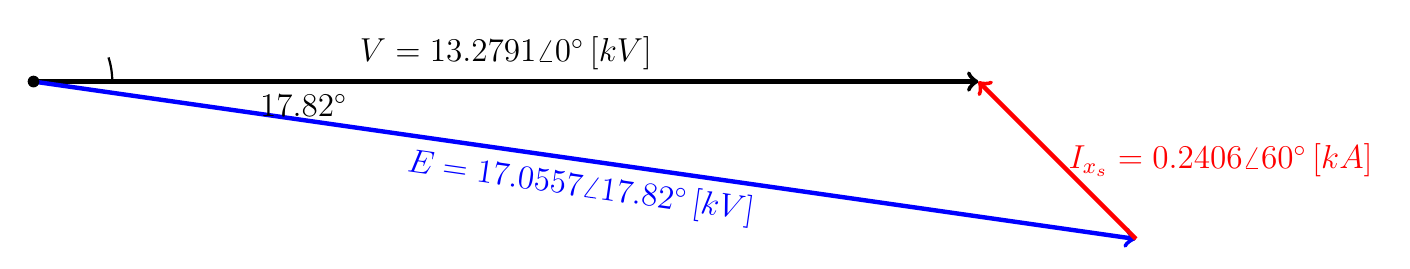
\begin{tikzpicture}

% Definir los puntos
\coordinate (O) at (0,0); % Origen
\coordinate (V) at (12,0); % Punto V
\coordinate (E) at (14,-2); % Punto E con el ángulo

% Dibujar las líneas
\draw[->, ultra thick, black] (O) -- (V) node[midway, above] {\large $V = 13.2791 \angle 0^\circ \, \text{[kV]}$}; % Línea V
\draw[->, ultra thick, blue] (O) -- (E) node[midway, below, sloped] {\large $E = 17.0557 \angle 17.82^\circ \, \text{[kV]}$}; % Línea E
\draw[->, ultra thick, red] (E) -- (V) node[midway, right] {\large $I_{x_s} = 0.2406 \angle 60^\circ \, \text{[kA]}$}; % Línea corriente

% Dibujar el ángulo con color negro y ajustar la ubicación del texto
\draw[thick] (1,0) arc[start angle=0,end angle=17.82,radius=1] node[above left, xshift=90, yshift=-25] {\large $17.82^\circ$};

% Añadir un punto para hacer el ángulo más visible
\node at (O) [circle,fill,inner sep=1.5pt] {};

\end{tikzpicture}
